%!Mode:: "TeX:UTF-8"
\documentclass[a4paper,11pt,UTF8]{ctexart}

\usepackage{indentfirst} %缩进
\usepackage{xeCJK}    %使用系统字体
\usepackage{fancyhdr} %自定义页眉页脚
\pagestyle{empty}                   %不设置页眉页脚
\usepackage{amsmath, amsthm, amssymb, amsfonts} %数学公式
\usepackage[a4paper,left=3cm,right=3cm,top=3cm,bottom=3cm]{geometry}
%\usepackage[tmargin=1in,bmargin=1in,lmargin=1.25in,rmargin=1.25in]{geometry}.
\usepackage{booktabs} %插入表格
\usepackage[section]{placeins} %避免浮动
\usepackage{listings} %插入代码
\usepackage{ctex}     %中文宏包
\usepackage[svgnames, table]{xcolor} %彩色表格
\usepackage{algorithm}          %伪代码
\usepackage{algorithmicx}
\usepackage{algpseudocode}
\usepackage{algorithm,algpseudocode,float}
\usepackage{lipsum}
\usepackage{enumitem}           %调整列举环境
\usepackage{url}
\usepackage{fontspec,xunicode}
\defaultfontfeatures{Mapping=tex-text} %如果没有它,会有一些 tex 特殊字符无法正常使用,比如连字符。

\usepackage{graphicx}
\graphicspath{{imgs/}}

%%%%%%%%%%%%%%%%%%%%%%%%%%%%%%%%%%%%%%%%%%%%%%%%%%%%%%%%%%%%%%%%
% 缩进及行间距
%%%%%%%%%%%%%%%%%%%%%%%%%%%%%%%%%%%%%%%%%%%%%%%%%%%%%%%%%%%%%%%%
\setlength{\parindent}{22pt} %重新定义缩进长度
\setlength{\baselineskip}{20pt}  %定义行间距
%\renewcommand{\baselinestretch}{1.1} %定义行间距

%%%%%%%%%%%%%%%%%%%%%%%%%%%%%%%%%%%%%%%%%%%%%%%%%%%%%%%%%%%%%%%%
% 列表设置
%%%%%%%%%%%%%%%%%%%%%%%%%%%%%%%%%%%%%%%%%%%%%%%%%%%%%%%%%%%%%%%%
\setenumerate{fullwidth,itemindent=\parindent,listparindent=\parindent,itemsep=0ex,partopsep=0pt,parsep=0ex}
\setenumerate[2]{label=\alph*),leftmargin=1.5em}  %二级item设置
\setitemize{itemindent=38pt,leftmargin=0pt,itemsep=-0.4ex,listparindent=26pt,partopsep=0pt,parsep=0.5ex,topsep=-0.25ex}
\setdescription{itemindent=38pt,leftmargin=0pt,itemsep=-0.4ex,listparindent=26pt,partopsep=0pt,parsep=0.5ex,topsep=-0.25ex}

%%%%%%%%%%%%%%%%%%%%%%%%%%%%%%%%%%%%%%%%%%%%%%%%%%%%%%%%%%%%%%%%
% 图的标题行间距设置
%%%%%%%%%%%%%%%%%%%%%%%%%%%%%%%%%%%%%%%%%%%%%%%%%%%%%%%%%%%%%%%%
\newcommand{\bottomcaption}{%
\setlength{\abovecaptionskip}{6pt}%
\setlength{\belowcaptionskip}{6pt}%
\caption}


%%%%%%%%%%%%%%%%%%%%%%%%%%%%%%%%%%%%%%%%%%%%%%%%%%%%%%%%%%%%%%%%
% 字体定义
%%%%%%%%%%%%%%%%%%%%%%%%%%%%%%%%%%%%%%%%%%%%%%%%%%%%%%%%%%%%%%%%
\setmainfont{Times New Roman}  %默认英文字体.serif是有衬线字体sans serif无衬线字体
\setmonofont{Consolas}
\setCJKmainfont[ItalicFont={楷体}, BoldFont={黑体}]{宋体}%衬线字体 缺省中文字体为
\setCJKsansfont{黑体}
\punctstyle{hangmobanjiao}
%-----------------------xeCJK下设置中文字体------------------------------%
\setCJKfamilyfont{song}{SimSun}                             %宋体 song
\newcommand{\song}{\CJKfamily{song}}
\setCJKfamilyfont{fs}{FangSong}                      %仿宋  fs
\newcommand{\fs}{\CJKfamily{fs}}
\setCJKfamilyfont{ktgb}{KaiTi}                      %楷体2312 ktgb
\newcommand{\ktgb}{\CJKfamily{ktgb}}
\setCJKfamilyfont{yh}{Microsoft YaHei}                    %微软雅黑 yh
\newcommand{\yh}{\CJKfamily{yh}}
\setCJKfamilyfont{hei}{SimHei}                              %黑体  hei
\newcommand{\hei}{\CJKfamily{hei}}
\setCJKfamilyfont{hwxk}{STXingkai}                                %华文行楷  hwxk
\newcommand{\hwxk}{\CJKfamily{hwxk}}
%------------------------------设置字体大小------------------------%
\newcommand{\shiyanbaogao}{\fontsize{36pt}{\baselineskip}\selectfont}
\newcommand{\chuhao}{\fontsize{42pt}{\baselineskip}\selectfont}     %初号
\newcommand{\xiaochuhao}{\fontsize{36pt}{\baselineskip}\selectfont} %小初号
\newcommand{\yihao}{\fontsize{28pt}{\baselineskip}\selectfont}      %一号
\newcommand{\erhao}{\fontsize{21pt}{\baselineskip}\selectfont}      %二号
\newcommand{\xiaoerhao}{\fontsize{18pt}{\baselineskip}\selectfont}  %小二号
\newcommand{\sanhao}{\fontsize{15.75pt}{\baselineskip}\selectfont}  %三号
\newcommand{\sihao}{\fontsize{14pt}{\baselineskip}\selectfont}       %四号
\newcommand{\xiaosihao}{\fontsize{12pt}{\baselineskip}\selectfont}  %小四号
\newcommand{\wuhao}{\fontsize{10.5pt}{\baselineskip}\selectfont}    %五号
\newcommand{\xiaowuhao}{\fontsize{9pt}{\baselineskip}\selectfont}   %小五号
\newcommand{\liuhao}{\fontsize{7.875pt}{\baselineskip}\selectfont}  %六号
\newcommand{\qihao}{\fontsize{5.25pt}{\baselineskip}\selectfont}    %七号

%%%%%%%%%%%%%%%%%%%%%%%%%%%%%%%%%%%%%%%%%%%%%%%%%%%%%%%%%%%%%%%%
% 图题字体大小相同
%%%%%%%%%%%%%%%%%%%%%%%%%%%%%%%%%%%%%%%%%%%%%%%%%%%%%%%%%%%%%%%%
\usepackage{caption}
\captionsetup{font={footnotesize}}   % footnotesize = 9pt
\captionsetup[lstlisting]{font={footnotesize}}

%%%%%%%%%%%%%%%%%%%%%%%%%%%%%%%%%%%%%%%%%%%%%%%%%%%%%%%%%%%%%%%%
% 重定义枚举编号为 1),2)...
%%%%%%%%%%%%%%%%%%%%%%%%%%%%%%%%%%%%%%%%%%%%%%%%%%%%%%%%%%%%%%%%
\renewcommand{\labelenumi}{\theenumi)}

%%%%%%%%%%%%%%%%%%%%%%%%%%%%%%%%%%%%%%%%%%%%%%%%%%%%%%%%%%%%%%%%
% 标题名称中文化
%%%%%%%%%%%%%%%%%%%%%%%%%%%%%%%%%%%%%%%%%%%%%%%%%%%%%%%%%%%%%%%%
\renewcommand\figurename{\hei 图}
\renewcommand\tablename{\hei 表}
\renewcommand\lstlistingname{\hei 代码}
\renewcommand{\algorithmicrequire}{\textbf{输入:}}
\renewcommand{\algorithmicensure}{\textbf{输出:}}
\newtheorem{define}{定义}

%%%%%%%%%%%%%%%%%%%%%%%%%%%%%%%%%%%%%%%%%%%%%%%%%%%%%%%%%%%%%%%%
% 代码设置
%%%%%%%%%%%%%%%%%%%%%%%%%%%%%%%%%%%%%%%%%%%%%%%%%%%%%%%%%%%%%%%%
\lstset{
 columns=fixed,
 numbers=left,                                        % 在左侧显示行号
 numberstyle=\tiny\color{gray},                       % 设定行号格式
 frame=single,                                        % 单线背景边框
 breaklines=true,                                     % 设定LaTeX对过长的代码行进行自动换行
 keywordstyle=\color[RGB]{40,40,255},                 % 设定关键字颜色
 numberstyle=\footnotesize\color{darkgray},
 commentstyle=\it\color[RGB]{0,96,96},                % 设置代码注释的格式
 stringstyle=\rmfamily\slshape\color[RGB]{128,0,0},   % 设置字符串格式
 showstringspaces=false,                              % 不显示字符串中的空格
 language=java,                                        % 设置语言
 basicstyle=\linespread{1.0}\xiaowuhao\ttfamily,                      % 字体字号
 %lineskip=10pt,
 %baselinestretch=1,
}

%%%%%%%%%%%%%%%%%%%%%%%%%%%%%%%%%%%%%%%%%%%%%%%%%%%%%%%%%%%%%%%%
% 伪代码分页
%%%%%%%%%%%%%%%%%%%%%%%%%%%%%%%%%%%%%%%%%%%%%%%%%%%%%%%%%%%%%%%%
\makeatletter
\renewcommand{\ALG@name}{算法}
\newenvironment{breakablealgorithm}
  {% \begin{breakablealgorithm}
   \begin{center}
     \refstepcounter{algorithm}% New algorithm
     \hrule height.8pt depth0pt \kern2pt% \@fs@pre for \@fs@ruled
     \renewcommand{\caption}[2][\relax]{% Make a new \caption
       {\raggedright\textbf{\ALG@name~\thealgorithm} ##2\par}%
       \ifx\relax##1\relax % #1 is \relax
         \addcontentsline{loa}{algorithm}{\protect\numberline{\thealgorithm}##2}%
       \else % #1 is not \relax
         \addcontentsline{loa}{algorithm}{\protect\numberline{\thealgorithm}##1}%
       \fi
       \kern2pt\hrule\kern2pt
     }
  }{% \end{breakablealgorithm}
     \kern2pt\hrule\relax% \@fs@post for \@fs@ruled
   \end{center}
  }
\makeatother

% =============================================
% Part 1 Edit the info
% =============================================

\newcommand{\major}{物理学院}
\newcommand{\name}{黄阅迅,李秋阳}
\newcommand{\stuid}{PB18020631,PB18020567}
\newcommand{\group}{20}
\newcommand{\newdate}{\today}
\newcommand{\p}{\par}
\newcommand{\np}{\par\noindent}

\newcommand{\course}{电子线路实验(1)}
\newcommand{\newtitle}{波形放大器}

% =============================================
% Part 1 Main document
% =============================================
\begin{document}
\thispagestyle{empty}
\begin{figure}[h]
  \begin{minipage}{0.6\linewidth}
    \centerline{
\includegraphics[width=\linewidth]{logo.png}}
  \end{minipage}
  \hfill
  \begin{minipage}{.4\linewidth}
    \raggedleft
    \begin{tabular*}{.8\linewidth}{ll}
      学院: & \underline\major   \\
      姓名: & \underline\name    \\
      学号: & \underline\stuid   \\
      组号:  & \underline\group   \\
      日期: & \underline\newdate \\
    \end{tabular*}
  \end{minipage}
\end{figure}

\begin{table}[!htbp]
  \centering
  \begin{tabular*}{\linewidth}{llllll}
    课程名称:  \underline\course   \qquad\qquad 实验题目:  \underline\newtitle  
  \end{tabular*}
\end{table}

% =============================================
% Part 2 Main document
% =============================================

\section{实验目的}

请参看预习报告。

\section{实验原理}

请参看预习报告。

\section{实验内容与步骤}
\subsection{实验内容一}
	搭建RC正弦波振荡器,并测量其相关性质。
\subsection{实验步骤一}
\begin{enumerate}
  \item 如图\ref{fig:RCSin}连接电路,调节电位器$R_W$,观察振荡器输出端$u_o$
  的波形,测量临界起振时正弦波的$R_W$值,并画出此时输出波形。
  \item 调节电位器$R_W$,使输出电压$U_o$幅值最大、稳定且不失真,画出输出波形,并测出相应的fo值。用交流毫
  伏表分别测量输出电压$U_o$和反馈电压$U_{p1}$的值。
  \item 改变$R_4=R_5=20kΩ$,电容$C_1,C_2$的值不变,测量并画出振荡器稳定输出波形,并测出相应fo的值。
\end{enumerate}
\begin{figure}[htbp]
  \centering
  \fbox{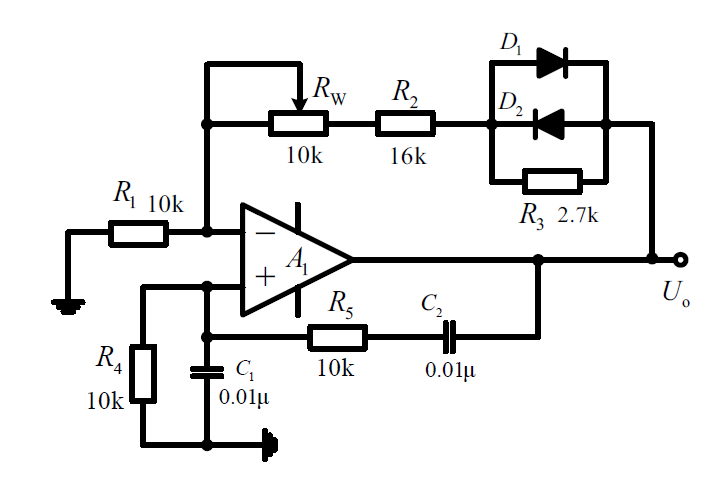
\includegraphics[width=0.5\linewidth]{RCSin.PNG}}
  \caption{RC正弦波振荡器实验电路图}
  \label{fig:RCSin}
  \end{figure}
\subsection{实验内容二}
	搭建方波-三角波发生器,并测量其输出波形,探讨频率幅度与电阻的关系。
\subsection{实验步骤}
\begin{enumerate}
  \item 如图\ref{fig:STWave}连接电路,将电位器调节到合适的位置,用双踪示波器观察并画出$u_{o1}$和$u_{o2}$的波形,测量其幅值、频
  率$f_o$的值(电位器$R_W=47kΩ$)。
  \item 电阻$R_1=10kΩ$,调节$R_W$,观察对$u_{o1},u_{o2}$幅值及fo的影响。
  \item 电位器$R_W=47kΩ$,改接电阻$R_1$为$10kΩ$电位器,调节$R_1$,观察对$u_{o1},u_{o2}$幅值及$f_o$的影响。
\end{enumerate}
\begin{figure}[htbp]
  \centering
  \fbox{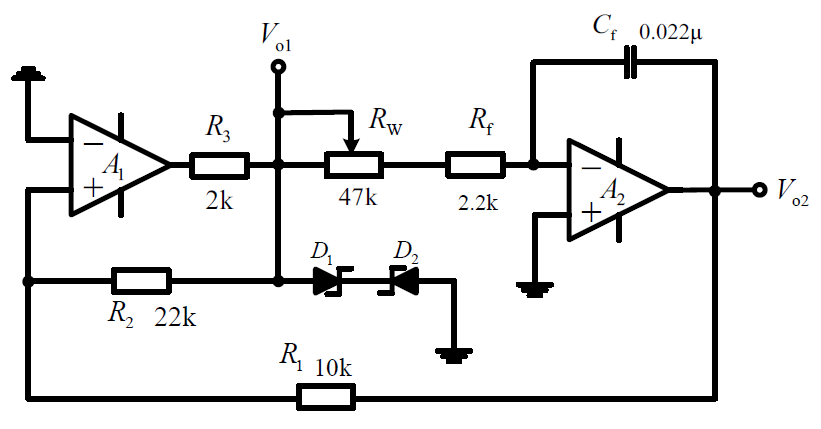
\includegraphics[width=0.5\linewidth]{STWave.PNG}}
  \caption{方波三角波实验电路图}
  \label{fig:STWave}
  \end{figure}

\section{实验数据处理与分析}
\subsection{实验内容1}
\begin{enumerate}
  \item 实验测量得到当$R_W=0.9026k\Omega$时,恰好产生震荡,此时测量得到的波形如附图一所示,测得频率值为
  $f_0=1.566kHz$
  \item 测得输出电压幅度最大且不失真时电阻为$R_W=1.617k\Omega$,$f_0=1.490kHz$,测量得到的波形图附图二所示,交流毫伏表测量得到的值为$U_{o}=5.69Vrms,U_{P1}=1.87Vrms$。
  \item 改变$R_4,R_5$的阻值后,测量得到的稳定输出波形如附图三所示,此时$f_0=737.04Hz$。
\end{enumerate}
\subsection{误差分析1}
  为分析误差,首先求出震荡频率的理论值,由于二极管的电阻不明,因此无法求出临界震荡电阻,有
  \begin{equation}
    \begin{aligned}
      f_0&=\frac{1}{2\pi RC}\\
      R&=R_4=R_5=10k\Omega\Rightarrow f_{01}=1.591kHz\\
      R&=R_4=R_5=20k\Omega\Rightarrow f_{02}=795.77Hz
    \end{aligned}
  \end{equation}
  由此,可见三次测量得到的相对误差分别为:
  \begin{equation}
    \left |\frac{\Delta f_{01}^{(0)}}{f_{01}}\right |=1.6\%,
    \left |\frac{\Delta f_{01}^{(1)}}{f_{01}}\right |=6.3\%,
    \left |\frac{\Delta f_{02}}{f_{02}}\right |=7.4\%,
  \end{equation}
  可见,误差相对较小,实验测量得到的频率值相比理论值均偏小,推测可能是$C_1$实际值比标称值偏大导致的。同时,
  示波器本身也带来一定的测量误差。但实验中发现实际上频率会随着$R_W$有一定的变化,虽然不大,但这与理论预言不符合。这是因为放大器
  本身并非理想,本身有一定的频率响应带来了一定的调制。
\subsection{实验内容2}
\begin{enumerate}
  \item 实验测量得到,当$R_W=43.62k\Omega$时,产生频率为$f_0=419Hz$的三角波,输出的波形图如附图四所示,可见三角波与方波反向,幅度比为$|A|=0.472$。
  \item 实验测量得到,当$R_W$增大时频率减小,反之增大。而$u_{o1},u_{o2}$幅度基本不变。
  \item 固定$R_W$,当$R_1$增大时,频率减小,$u_{o2}$增大;反之频率增大,$u_{o2}$减小。$u_{o1}$幅度基本不变。
\end{enumerate}
\subsection{误差分析2}
  理论求出输出频率以及幅度比如下:
  \begin{equation}
    \begin{aligned}
      f_0&=\frac{R_2}{4R_1(R_W+R_f)C}=540Hz\\
      |A|&=\frac{R_1}{R_2}=0.454
    \end{aligned}
  \end{equation}
  则可以求出相对误差分别为:
  \begin{equation}
    \left |\frac{\Delta f_{0}}{f_{0}}\right |=22.4\%,
    \left |\frac{\Delta A}{A}\right |=4.0\%,
  \end{equation}
  可见频率的误差很大,经检测,反馈电容实际值为$C_f=28nF$,对应理论频率$f_0=424Hz,\left |\frac{\Delta f_{0}}{f_{0}}\right |=1.2\%$,可见这个误差主要是因为反馈电容$C_f$的值与标识值误差很大造成的。
  幅度比值误差较小,实验结果比较理想。

  同时,从理论分析中,可以知道$R_W$增大时,$f_0$的分母增大,故$f_0$减小,而$|A|$与$R_W$无关。因此,实验得到的变化趋势与理论分析吻合。
  当$R_1$增大时,同样有$f_0$的分母增大,故$f_0$减小。同时$|A|$的分母也增大,因此$|A|$也减小,当$u_{o1}$不变时,$|u_{o2}|$减小,均与理论吻合。误差主要来源于元件的
  标识值误差,同时也有示波器的测量误差。
\section{实验总结}
本次实验通过搭建RC桥式正弦波振荡器电路和方波三角波发生器电路,学习了震荡电路的基本构成,原理和实验方法。并利用示波器测量了其相关的性能以及性质。总体
实验结果与理论吻合得较好,虽然有一定误差,但也准确地定位了误差的来源,做了修正。
\section{实验思考题}
 \subsection{RC正弦波振荡器电路中,二极管 $D_1$、$D_2$ 在电路中起什么作用,说明它们的工作原理。}
 \np \textbf{答:}两个二极管正反并联,这样只要两端电压的绝对值大于二极管开启电压(比如典型值0.7V),那么就会被钳位,电压绝对值无法继续提高。
 \p 在起振阶段,电压幅值很小,没有超过二极管开启电压,二极管截止,电阻 $R_F$ 比较大,因此
 \[ A=\left( 1+\frac{R_F}{R_1} \right)>3 \]
 这样 $AF>1$,电压会被不断放大,达到起振的效果。
 \p 而在电压达到一定幅值之后,二极管开启,阻值 $R_F$ 下降,此时
 \[ A=\left( 1+\frac{R_F}{R_1} \right)\to3 \]
 这样较大的电压会逐步稳定,直至 $AF=1$ 完全成立,幅值不再改变,于是产生了稳定的正弦波。
 \subsection{三角波的输出幅度是否可以超过方波的幅度?如果运放的正负电源不等,输出波形如何?}
 \textbf{答:}三角波的幅度不可以超过方波,否则发生失真,理由如下:
 \p 整个系统的周期为$T=\frac{4R_1(R_w+R_f)C}{R_2}$。而积分电路要求$\frac{T}{2}<\tau$。
 \p 综合上述二式得到:$\frac{R_1}{R_2}<0.5$。即$\frac{V_{o2m}}{V_z}=\frac{R_1}{R_2}<0.5$
 \p 假如运放的正负电压不一样,那么运放的输入输出曲线的正负饱和区不对称,于是滞回比较器的门限电压也不关于0对称。那么三角波的正负端电压也不对称。不过由于稳压对管的限制,方波的电压应该是不会变的。


\end{document}
